%%% EtherPad for Discrete Mathematics VO
%%% http://www.informatik-forum.at/showthread.php?104454-Notes-2013WS-VO_01
%%% Past pads:
%%%     * 2013-10-17: committed by patrikf
%%%     * 2013-10-18: committed by patrikf

% Discrete Mathematics Lecture Notes 2013-10-24

% clarification of last week

$G$ planar multigraph
$G*= (V*, E*), V*= F$
$E*: $ for every edge $e \in E$ set $e* = f_1 f_2$ if $f_1$, $f_2$ are the facs "left" and "right" of $e$

\TODO{ G}
%plot

\textbf{Remark:}
1) |E| = |E*|
2) In general |G*| is a multigraph
3) $G_1, G_2$ are duals of $G \Rightarrow G_1 \cong G_2$

$A \subeq E$    
$A$ cycle in $G \iff A*$ minimal cut

If G is not necessarily planar: define $G*$ by (*)
This Graph is uniqe, if it exists (combinor

\textbf{Theorem (Witness Theorem).} \\
If G is not necessarily planar: define $G**$ by (*)
* $G$ planar $\Rightarrow G** \cong G*$
* $G$ non planar $\not\exists G**$

% end of last weeks-corrections


\subsection*{Matchings and Bipartite Graphs}

\textbf{Theorem (Hall's marriage theorem).}
$W, M$ (women, men) vertex set of a bipartite graph
($V=W\cup M$, $wm \in E \iff wFm$). $W,M$ finite, nonempty, $W\cap M=\varnothing$.

Friendship relation $F\subseteq W\times M$.

Feasible marriage: complete matching $F_1\subseteq F$, i.e.
\[ \forall x\in W: \exists! y\in M\text{ s.t. }x\operatorname{F} y \]

Theorem: There is a feasible marriage iff
\[
    \forall W_0\subseteq W:
        \underbrace{
            |\{y\in M\mid \exists x\in W_0: x\operatorname{F} y\}|
        }_{\Cup_{w\in W_0} \Gamma(w)}
        ≥ |W_0|
\]

if you have a feasable marriage, every woman gets a partner.
The Set of friends is at least this large

\textbf{Proof.}
Consider the network source $s$ $\rightarrow_{w=1}$ women $\rightarrow_{w=|W|+|M|+1}$ men $\rightarrow_{w=1}$ sink $t$.
Since all weights are integer, $\exists$ maximal flow with integer weight.
\TODO{add plot describing the nework}

We claim that $S=(\{s\}, V \setminus \{s\})$
is a minimal cut ($c(S) = |W|$).

Assume $\exists S': c(S') < c(s)$. Then $S'$ has no edge $wm$ with $w\in W, m\in M$.

\[
S' = (V_1,V_2) ^=
    \{sw\mid w \in \widetilde{W} \subseteq W \} \cup
    \{mt | m \in \widetilde{M} \subset M \}
\]

We claim that
\[
    w\in W\setminus\widetilde{W}, m\in\GammaPlus(w)
    \implies m\in\widetilde{M}.
\]
Assume this does not hold. Then
\path{s, w, m, t} does not contain an edge of $S'$ $\implies s, t\in V_1$. Contradiction!

This implies that
\[
    |\Cup_{w\in W\setminus\widetilde{W}} \GammaPlus(w)|
    ≤ |\widetilde{M}|.
\]
But
\[
    c(S') = |\widetilde{W}| + |\widetilde{M}| < c(S) = |W|.
\]
This implies that
\[
    |\widetilde{M}| < |W\setminus \widetilde{W}|.
\]
Contradiction! Therefore $S'$ can not be a minimal cut. $S$ is proven to be a minimal cut.

The theorem of Ford-Fulkerson says that with a minimal cut,
$\exists\;\text{flow }\phi: v(\phi) = c(S) = |W|$. This flow defines the feasible marriage relation.


\subsection*{Graph Colorings}

\begin{definition}
$G=(V,E)$ simple, undirected graph.
A \dt{vertex coloring} is a mapping
\[
    c : V\mapsto C, C=\{c_1,\ldots,c_r\}
\].
A coloring is \dt{feasible} if $vw\in E\implies c(v)≠c(w)$.
\end{definition}

\Remark. Edge coloring $\bar{c}: E\mapsto C$, feasible if edges with a common vertex have different colors.

\bar{G} = (\bar V, \bar E), \bar V = E
e_1 e_2\in \bar E \iff e_1,e_2\text{ share common vertex}

\Remark. Similarly, face colorings of a planar graph (think of a map of countries) can be 

\begin{definition}
$G=(V,E)$ graph. The \dt{chromatic number} $\chi(G)$ is the minimal number of colors so that there is a feasible coloring.
\end{definition}

Examples:
$\chi(K_n) = n$

$\chi(K_{n,m}) = 2$

$\chi(T) = 2$ if $T$ tree, $|V| ≥ 1$.

\Theorem.
\[
\begin{array}{r@{\quad}r@{ }l}
\text{1.} &
    \chi(G) = 1&\iff E(G) = \varnothing. \\
\text{2.} &
    \chi(G) = 2
        &\iff E(G) ≠ \varnothing, G\text{ bipartite} \\
        &&\iff E(G) ≠ \varnothing, \text{all cycles have even length}
\end{array}
\]

\Theorem.
$G$ planar $\implies \chi(G) \leq 4$. Proof is very hard!

\Theorem.
$\chi(G) ≤ 1 + \max{d(v)}.$

\Proof. By induction on $\alpha_0(G)$.

\Theorem. $G$ planar$\implies \chi(G) ≤ 5$.

\def\dmin{\ensuremath{d_{\text{min}}}}
\Proof.
Claim: In a planar graph, all vertices have at most five neighbors:
$\dmin ≤ 5$.

Assume $\dmin ≥ 6$.
Then
$2\alpha_1 = \sum_{x\in V} d(x) ≥ 6\alpha_0$
\alpha_1 ≥ \alpha_0.

2\alpha_1 ≥
\sum_{\text{faces}} \text{number of boundary edges} ≥
3\alpha_2 =
3 (2 - \alpha_0 + \alpha_1)

\alpha_1 ≤ 3\alpha_0 - 6

But $\alpha_1 ≥ 3\alpha_0$! Contradiction.

Case 1:
$\dmin \leq 4$. Pick $x_0$ so that $d(x_0) \leq 4$.
Take $G' = G \setminus \{x_0\}$. Assume $\chi(G')=5$. Then, since $x_0$ has at most $4$ neighbors, you can color $x_0$ with the remaining color. By induction, $\chi(G)=5$.

Case 2:
$d_{\text{min}}=5$.
We have a vertex $v$ with exactly 5 neighbours $\{a,b,c,d,e\}$.
$c(a) = 1, c(b) = 2,\ldots$.

$G_a = \{x\in V\mid \exists 1--3--1--3--\ldots path a \leadsto x\}$.
Similar for $G_c$.
Case 2.1: If $G_a\cap G_c =\varnothing$, we can recolor $G_a$ by switching colors 1 and 3. Then we can color $v$ with $c(v) = 1$.

Case 2.2: If $G_a\cap G_c ≠\varnothing$, then $G_a = $G_c$.
Case 2.2.1: If $G_b\cap G_d =\varnothing$, then recolor $G_b$ by switching 2 and 4, and $c(v) = 2.
Case 2.2.2: If $G_b\cap G_d ≠\varnothing$, then $G_b = G_d$. Contradiction! (planar graph - the paths $G_a=G_c$ and $G_b=G_d$ cannot cross each other)


\subsection*{Ramsey Theory}

\textbf{Example.} Every 2-edge coloring of $K_6$ has a monochromatic $K_3$.

\TODO{format figure $K_6$ $K_3$}
% \begin{figure}
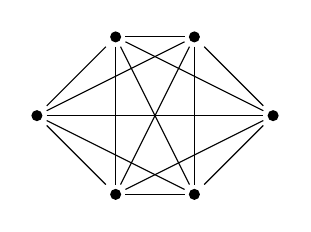
\begin{tikzpicture}
  \node (n1) at (0,1) {};
  \node (n2) at (1,2) {};
  \node (n3) at (2,2) {};
  \node (n4) at (3,1) {};
  \node (n5) at (2,0) {};
  \node (n6) at (1,0) {};

  \foreach \i in {1,...,6}
  {
    \fill (n\i) circle(2pt);
    \foreach \j in {\i,...,6}
    {
      \path (n\i) edge (n\j);
    };
  };
\end{tikzpicture}

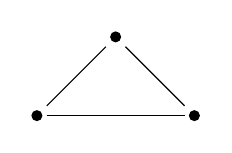
\begin{tikzpicture}
  \node (n1) at (0,0) {};
  \node (n2) at (1,1) {};
  \node (n3) at (2,0) {};

  \foreach \i in {1,...,3}
  {
    \fill (n\i) circle(2pt);
    \foreach \j in {\i,...,3}
    {
      \path (n\i) edge (n\j);
    };
  };
\end{tikzpicture}

% \end{figure}

\TODO{Proof (graphical).}

\begin{definition}
The Ramsey number $R(r,s)$ is
\[
    R(r,s) =
        min \{n\mid \text{every red-blue coloring of $K_n$ contains a red $K_r$ or a blue $K_s$}\}.
\]
\end{definition}

By our example, $R(3,3) ≤ 6$. We can even show that $R(3,3) = 6$.

\TODO{figure $K_5$}

Lemma. R(r,s) ≤ R(r-1, s) + R(r, s-1)

Proof. n = R(r-1, s) + R(r, s-1)
Partition $K_n$. Take a vertex $v$. All neighbours connected by a red edge are in $M$; all neighbours connected by a red edge are in $N$.
n = |M|+|N|+1. Thus
|M| ≥ R(r-1, s) or |N| ≥ R(R, s-1).

Case 1: \exists blue K_s in M or \exists red K_{r-1} in M.
Case 2: \exists blue K_{s-1} or red K_r in N.

We wanted to show that \exists blue K_s or \exists red K_r.
In both cases, \emph{together with $v$}, we can always find a blue K_s or a red K_r.

\Corollary. R(r,s) ≤ \choose{r+s-2}{r-1} ≤ 2^{r+s-2}

\Proof. R(2,n) = R(n,2) = n ≤ \choose{n}{1}. From there, apply induction, Pascal's triangle, and the above lemma.

\begin{definition}
\[
    R(n_1,n_2,\ldots,n_r) =
    \min \{ n \mid
        \text{all r-edge colorings of $K_n$
        (colors $c_1,\ldots,c_r$) have a
        $c_j$-colored $K_j$ for some j}
\]
\end{definition}











